% Created 2022-12-08 Thu 09:20
% Intended LaTeX compiler: pdflatex
\documentclass[11pt]{article}
\usepackage[utf8]{inputenc}
\usepackage[T1]{fontenc}
\usepackage{graphicx}
\usepackage{longtable}
\usepackage{wrapfig}
\usepackage{rotating}
\usepackage[normalem]{ulem}
\usepackage{amsmath}
\usepackage{amssymb}
\usepackage{capt-of}
\usepackage{hyperref}
\author{Rafał Grot}
\date{\today}
\title{Matma}
\hypersetup{
 pdfauthor={Rafał Grot},
 pdftitle={Matma},
 pdfkeywords={},
 pdfsubject={},
 pdfcreator={Emacs 28.2.50 (Org mode 9.6)}, 
 pdflang={English}}
\begin{document}

\maketitle
\tableofcontents


\section{liczby zespolone}
\label{sec:org171be63}
\begin{itemize}
\item \(\mathbb{Z}\) -- zbiór liczb całkowitych
\item \(\mathbb{R}\) -- zboór liczb rzeczywistych
\item \(\mathbb{C}\) -- zbiór liczb zespolonych
\end{itemize}
$$\mathbb{Z} \subset \mathbb{R} \subset \mathbb{C}$$
\subsection{postać algerbraiczna liczby zespolonej}
\label{sec:org6f62e4c}
$$z=a+bi$$

\begin{itemize}
\item \(\Re(z) = a\) -- część rzeczywista liczby zespolonej.
\item \(\Im(z) = b\) -- częśc urojona liczby zespolonej.
\item \(i\) - jednostka urojona \(i^2=-1\)
\end{itemize}
\subsubsection{sprzężenie liczby zespolonej}
\label{sec:orged29b16}
\begin{latex}
\begin{align*}
  z=a+bi && \overline{z}=a-bi \\
  w=f-gi && \overline{w}=f+gi \\
\end{align*}
\end{latex}

\subsection{postać trygonometryczna liczby zespolonej}
\label{sec:org4b3c418}
$$z=(z)(\cos\varphi \cdot \sin\varphi)$$
\subsection{postać wykładnicza liczby zespolonej}
\label{sec:orgadbd8d5}
$$z=(z) \cdot e^{i\varphi}$$
\subsection{moduł liczby zespolonej}
\label{sec:orgbe55af4}

\begin{center}
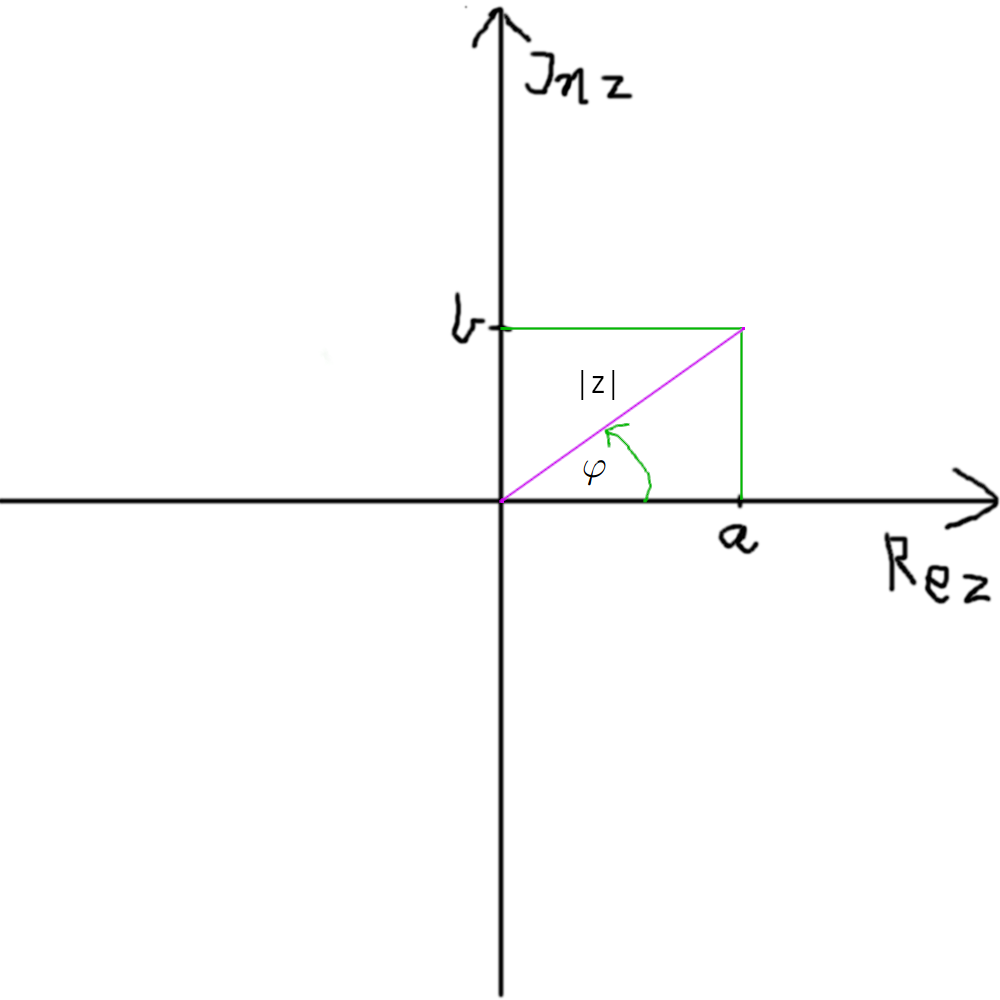
\includegraphics[width=.9\linewidth]{lzespolona.png}
\end{center}

$$|z|=\sqrt{a^2+b^2}$$

\(\varphi\) -- argument

\subsection{funkcja kwadratowa}
\label{sec:org3e30075}
$$z^2+z+1=0$$
\(\Delta = b^2-4ac = -3\) -- brak rozwiązań w \(\mathbb{R}\)
$$\sqrt{\Delta} = \sqrt{-3} = \sqrt{(-1)3} = \sqrt{-1}  \sqrt{3} = \sqrt{i^2}\sqrt{3} = i \sqrt{3} $$
$$z_1 = \frac{-b - \sqrt{\Delta} }{2a} \lor z_2=\frac{-b + \sqrt{\Delta} }{2a}$$
$$z_1 = \frac{-1-i\sqrt{3}}{2} = -\frac{1}{2} + \frac{\sqrt{3}}{2}i \lor
z_2 = \frac{-1 + i\sqrt{3}}{2} = - \frac{1}{2}+ \frac{\sqrt{3}}{2}i $$
\subsection{Potęgowanie liczby zespolonej}
\label{sec:org495b718}
$$z=a+bi \to z=|z|(\cos \varphi + i \sin \varphi)^n \to |z|^n(\cos n \varphi + i \sin n \varphi)$$

\section{Stożkowe}
\label{sec:org34339ee}
\[Q(\vec{x}) = a_{11}x_1^2 + 2a_{12}x_1x_2+a_{22}x_2^2
\to M =
\begin{bmatrix}
    a_{11} & a_{12}\\
    a_{21} & a_{22}\\
\end{bmatrix}\]

\[\det{M}\] -- wyróżnik formy kwadratowej \(Q(\vec{x})\)

\begin{latex}
\begin{align*}
  \det{M} &> 0 && \text{forma kwadratowa typu eliptycznego}\\
  \det{M} &= 0 && \text{forma kwadratowa typu parabolicznego}\\
  \det{M} &< 0 && \text{forma kwadratowa typu hiperbolicznego}\\
\end{align*}
\end{latex}

\subsection{Sprowadzanie do postaci kwadratowej}
\label{sec:orgc00a8ed}

\[Q(\vec{x}) = a_{11}x_1^2 + 2a_{12}x_1x_2+a_{22}x_2^}
\to
 Q(\vec{x}) = a_{1} \hat{x}_{1}^{2} + a_{2}\hat{x}_2^{2}\]

gdzie \(a_{1}, a_{2}\) -- wartości własne macierzy \(M\)

\(\hat{x}_1,\hat{x}_{2}\) -- współżędne wektora \(\vec{x}\) w nowej baze ortonormalnej \(\vec{v_{1}}, \vec{v_{2}}\) złożonej z wersorów własnych macierzy \(M\).

wersor własny -- wektor własny o długości 1.
\section{\(\mathbb{R}^3\)}
\label{sec:orgf2cd2ee}
\subsection{Równianie ogólne płaszczyzny}
\label{sec:org54afc7f}

\begin{center}
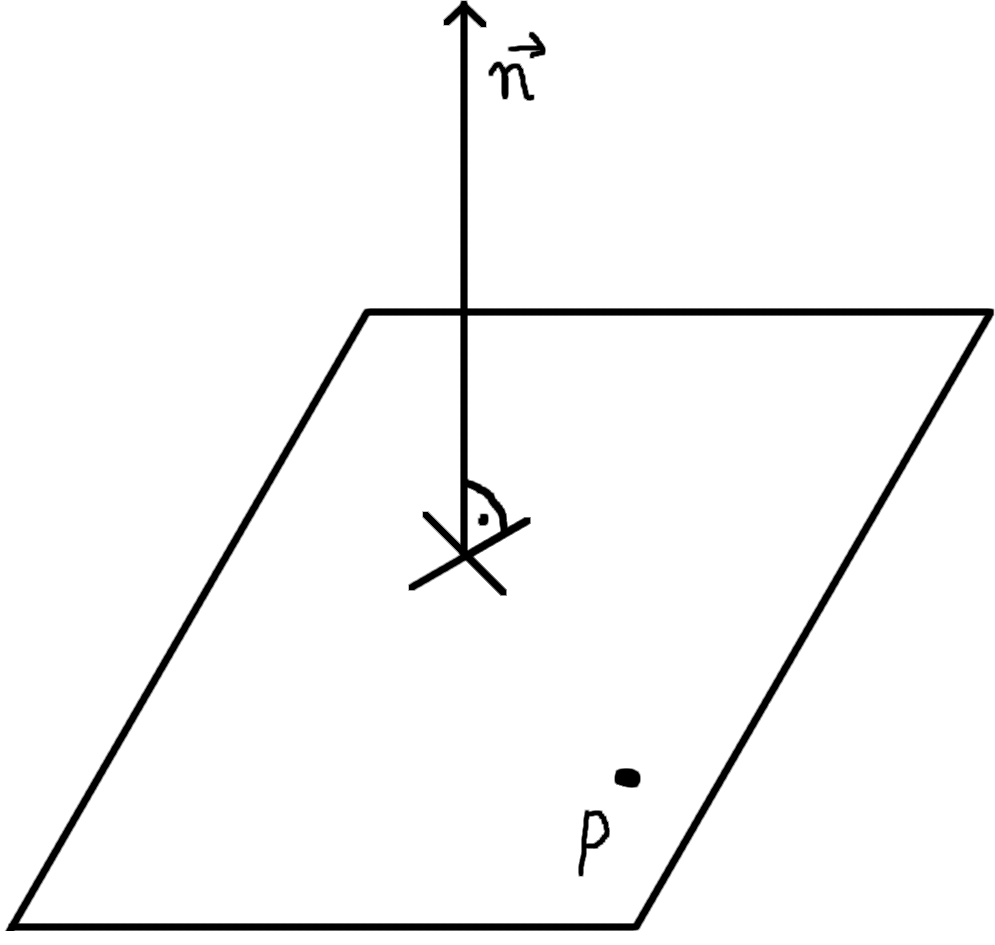
\includegraphics[width=.9\linewidth]{figures/plaszczyzna.png}
\end{center}

\begin{latex}
\begin{align*}
\vec{n}=[A,B,C] && P=(x_{0}, y_{0}, z_{0})
\end{align*}
\end{latex}

$$A(x - x_{0}) + B(y-y_{0}) + C(z - z_{0}) = 0$$
\end{document}